% Options for packages loaded elsewhere
\PassOptionsToPackage{unicode}{hyperref}
\PassOptionsToPackage{hyphens}{url}
%
\documentclass[
]{article}
\title{Meeting 7 Notes}
\author{Daniel Lupercio}
\date{3/24/2022}

\usepackage{amsmath,amssymb}
\usepackage{lmodern}
\usepackage{iftex}
\ifPDFTeX
  \usepackage[T1]{fontenc}
  \usepackage[utf8]{inputenc}
  \usepackage{textcomp} % provide euro and other symbols
\else % if luatex or xetex
  \usepackage{unicode-math}
  \defaultfontfeatures{Scale=MatchLowercase}
  \defaultfontfeatures[\rmfamily]{Ligatures=TeX,Scale=1}
\fi
% Use upquote if available, for straight quotes in verbatim environments
\IfFileExists{upquote.sty}{\usepackage{upquote}}{}
\IfFileExists{microtype.sty}{% use microtype if available
  \usepackage[]{microtype}
  \UseMicrotypeSet[protrusion]{basicmath} % disable protrusion for tt fonts
}{}
\makeatletter
\@ifundefined{KOMAClassName}{% if non-KOMA class
  \IfFileExists{parskip.sty}{%
    \usepackage{parskip}
  }{% else
    \setlength{\parindent}{0pt}
    \setlength{\parskip}{6pt plus 2pt minus 1pt}}
}{% if KOMA class
  \KOMAoptions{parskip=half}}
\makeatother
\usepackage{xcolor}
\IfFileExists{xurl.sty}{\usepackage{xurl}}{} % add URL line breaks if available
\IfFileExists{bookmark.sty}{\usepackage{bookmark}}{\usepackage{hyperref}}
\hypersetup{
  pdftitle={Meeting 7 Notes},
  pdfauthor={Daniel Lupercio},
  hidelinks,
  pdfcreator={LaTeX via pandoc}}
\urlstyle{same} % disable monospaced font for URLs
\usepackage[margin=1in]{geometry}
\usepackage{color}
\usepackage{fancyvrb}
\newcommand{\VerbBar}{|}
\newcommand{\VERB}{\Verb[commandchars=\\\{\}]}
\DefineVerbatimEnvironment{Highlighting}{Verbatim}{commandchars=\\\{\}}
% Add ',fontsize=\small' for more characters per line
\usepackage{framed}
\definecolor{shadecolor}{RGB}{248,248,248}
\newenvironment{Shaded}{\begin{snugshade}}{\end{snugshade}}
\newcommand{\AlertTok}[1]{\textcolor[rgb]{0.94,0.16,0.16}{#1}}
\newcommand{\AnnotationTok}[1]{\textcolor[rgb]{0.56,0.35,0.01}{\textbf{\textit{#1}}}}
\newcommand{\AttributeTok}[1]{\textcolor[rgb]{0.77,0.63,0.00}{#1}}
\newcommand{\BaseNTok}[1]{\textcolor[rgb]{0.00,0.00,0.81}{#1}}
\newcommand{\BuiltInTok}[1]{#1}
\newcommand{\CharTok}[1]{\textcolor[rgb]{0.31,0.60,0.02}{#1}}
\newcommand{\CommentTok}[1]{\textcolor[rgb]{0.56,0.35,0.01}{\textit{#1}}}
\newcommand{\CommentVarTok}[1]{\textcolor[rgb]{0.56,0.35,0.01}{\textbf{\textit{#1}}}}
\newcommand{\ConstantTok}[1]{\textcolor[rgb]{0.00,0.00,0.00}{#1}}
\newcommand{\ControlFlowTok}[1]{\textcolor[rgb]{0.13,0.29,0.53}{\textbf{#1}}}
\newcommand{\DataTypeTok}[1]{\textcolor[rgb]{0.13,0.29,0.53}{#1}}
\newcommand{\DecValTok}[1]{\textcolor[rgb]{0.00,0.00,0.81}{#1}}
\newcommand{\DocumentationTok}[1]{\textcolor[rgb]{0.56,0.35,0.01}{\textbf{\textit{#1}}}}
\newcommand{\ErrorTok}[1]{\textcolor[rgb]{0.64,0.00,0.00}{\textbf{#1}}}
\newcommand{\ExtensionTok}[1]{#1}
\newcommand{\FloatTok}[1]{\textcolor[rgb]{0.00,0.00,0.81}{#1}}
\newcommand{\FunctionTok}[1]{\textcolor[rgb]{0.00,0.00,0.00}{#1}}
\newcommand{\ImportTok}[1]{#1}
\newcommand{\InformationTok}[1]{\textcolor[rgb]{0.56,0.35,0.01}{\textbf{\textit{#1}}}}
\newcommand{\KeywordTok}[1]{\textcolor[rgb]{0.13,0.29,0.53}{\textbf{#1}}}
\newcommand{\NormalTok}[1]{#1}
\newcommand{\OperatorTok}[1]{\textcolor[rgb]{0.81,0.36,0.00}{\textbf{#1}}}
\newcommand{\OtherTok}[1]{\textcolor[rgb]{0.56,0.35,0.01}{#1}}
\newcommand{\PreprocessorTok}[1]{\textcolor[rgb]{0.56,0.35,0.01}{\textit{#1}}}
\newcommand{\RegionMarkerTok}[1]{#1}
\newcommand{\SpecialCharTok}[1]{\textcolor[rgb]{0.00,0.00,0.00}{#1}}
\newcommand{\SpecialStringTok}[1]{\textcolor[rgb]{0.31,0.60,0.02}{#1}}
\newcommand{\StringTok}[1]{\textcolor[rgb]{0.31,0.60,0.02}{#1}}
\newcommand{\VariableTok}[1]{\textcolor[rgb]{0.00,0.00,0.00}{#1}}
\newcommand{\VerbatimStringTok}[1]{\textcolor[rgb]{0.31,0.60,0.02}{#1}}
\newcommand{\WarningTok}[1]{\textcolor[rgb]{0.56,0.35,0.01}{\textbf{\textit{#1}}}}
\usepackage{graphicx}
\makeatletter
\def\maxwidth{\ifdim\Gin@nat@width>\linewidth\linewidth\else\Gin@nat@width\fi}
\def\maxheight{\ifdim\Gin@nat@height>\textheight\textheight\else\Gin@nat@height\fi}
\makeatother
% Scale images if necessary, so that they will not overflow the page
% margins by default, and it is still possible to overwrite the defaults
% using explicit options in \includegraphics[width, height, ...]{}
\setkeys{Gin}{width=\maxwidth,height=\maxheight,keepaspectratio}
% Set default figure placement to htbp
\makeatletter
\def\fps@figure{htbp}
\makeatother
\setlength{\emergencystretch}{3em} % prevent overfull lines
\providecommand{\tightlist}{%
  \setlength{\itemsep}{0pt}\setlength{\parskip}{0pt}}
\setcounter{secnumdepth}{-\maxdimen} % remove section numbering
\ifLuaTeX
  \usepackage{selnolig}  % disable illegal ligatures
\fi

\begin{document}
\maketitle

\hypertarget{from-our-previous-meeting-i-have-atempted-some-arima-models-that-were-mentioned-in-the-duke-university-arima-guide.-the-basic-models-were-used-and-i-ultimately-felt-comfortable-adding-ma-arguments-to-the-dataset}{%
\section{\texorpdfstring{From our previous meeting, I have atempted some
ARIMA models that were mentioned in the
\href{https://people.duke.edu/~rnau/411arim2.htm}{DUKE} university ARIMA
guide. The basic models were used and I ultimately felt comfortable
adding MA() arguments to the
dataset}{From our previous meeting, I have atempted some ARIMA models that were mentioned in the DUKE university ARIMA guide. The basic models were used and I ultimately felt comfortable adding MA() arguments to the dataset}}\label{from-our-previous-meeting-i-have-atempted-some-arima-models-that-were-mentioned-in-the-duke-university-arima-guide.-the-basic-models-were-used-and-i-ultimately-felt-comfortable-adding-ma-arguments-to-the-dataset}}

\begin{Shaded}
\begin{Highlighting}[]
\CommentTok{\# save(bx\_ts, bx\_ts2, file = "BX\_ts.RData")}
\FunctionTok{load}\NormalTok{(}\StringTok{"meeting\_6.RData"}\NormalTok{)}
\end{Highlighting}
\end{Shaded}

\hypertarget{arima000-with-constant}{%
\subsubsection{ARIMA(0,0,0) with
constant}\label{arima000-with-constant}}

\begin{Shaded}
\begin{Highlighting}[]
\NormalTok{bx\_arima000\_fit }\OtherTok{\textless{}{-}}\NormalTok{ bx\_ts }\SpecialCharTok{\%\textgreater{}\%} \FunctionTok{model}\NormalTok{(}\AttributeTok{arima000\_constant =} \FunctionTok{ARIMA}\NormalTok{(total\_waste }\SpecialCharTok{\textasciitilde{}} \DecValTok{1} \SpecialCharTok{+} \FunctionTok{pdq}\NormalTok{(}\DecValTok{0}\NormalTok{,}\DecValTok{0}\NormalTok{,}\DecValTok{0}\NormalTok{)))}
\end{Highlighting}
\end{Shaded}

\begin{Shaded}
\begin{Highlighting}[]
\NormalTok{bx\_arima000\_fit}\SpecialCharTok{\%\textgreater{}\%} \FunctionTok{gg\_tsresiduals}\NormalTok{(}\AttributeTok{lag =} \DecValTok{24}\NormalTok{)}
\end{Highlighting}
\end{Shaded}

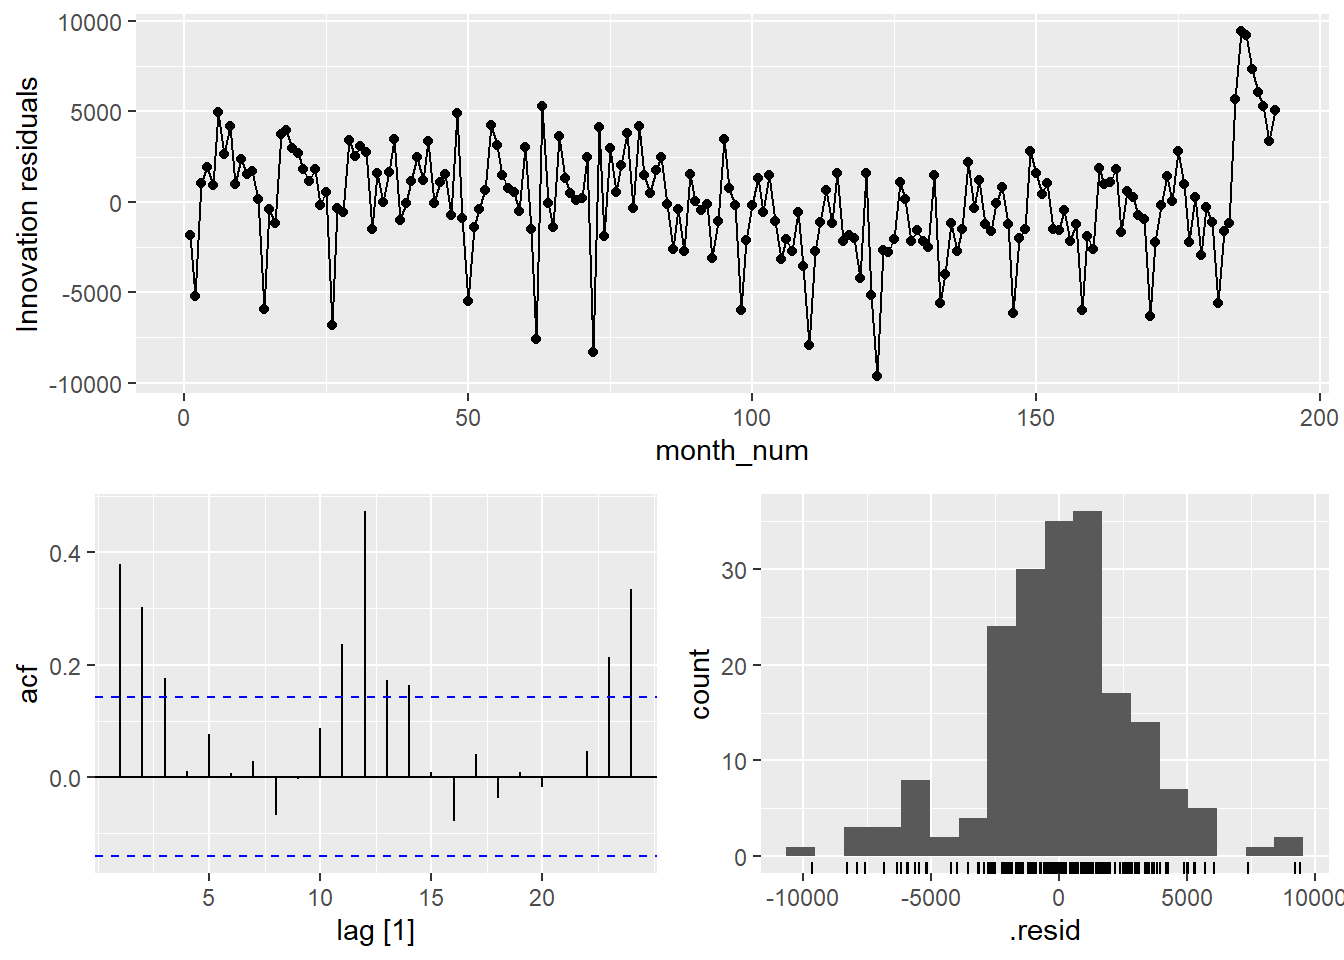
\includegraphics{final_sixth_meetings_notes_files/figure-latex/acf and resduals plot-1.pdf}
We can only see the PACF of the time series (tsibble), not of the model.

\begin{Shaded}
\begin{Highlighting}[]
\NormalTok{bx\_ts }\SpecialCharTok{\%\textgreater{}\%} \FunctionTok{gg\_tsdisplay}\NormalTok{(total\_waste, }\AttributeTok{plot\_type =} \StringTok{"partial"}\NormalTok{)}
\end{Highlighting}
\end{Shaded}

\includegraphics{final_sixth_meetings_notes_files/figure-latex/PACF and ACF plot-1.pdf}
From the ACF, we see significant lag spikes at lags (1,2, 3, 11, 12).

From the PACF, we see significant lag spikes at lags (1, 2, 11, 12 and
13). The first instance where the PACF ``cuts off'' is at lag 3.
Although the lag 1 of the PACF is not close to 1, it is unclear if
differencing is needed.

\hypertarget{arima100-with-no-constant}{%
\subsection{ARIMA(1,0,0) with no
constant}\label{arima100-with-no-constant}}

\begin{Shaded}
\begin{Highlighting}[]
\NormalTok{bx\_arima100\_fit }\OtherTok{\textless{}{-}}\NormalTok{ bx\_ts }\SpecialCharTok{\%\textgreater{}\%} \FunctionTok{model}\NormalTok{(}\AttributeTok{arima100\_constant =} \FunctionTok{ARIMA}\NormalTok{(total\_waste }\SpecialCharTok{\textasciitilde{}}  \FunctionTok{pdq}\NormalTok{(}\DecValTok{1}\NormalTok{,}\DecValTok{0}\NormalTok{,}\DecValTok{0}\NormalTok{)))}
\NormalTok{bx\_arima100\_fit }\SpecialCharTok{\%\textgreater{}\%} \FunctionTok{gg\_tsresiduals}\NormalTok{(}\AttributeTok{lag =} \DecValTok{24}\NormalTok{)}
\end{Highlighting}
\end{Shaded}

\includegraphics{final_sixth_meetings_notes_files/figure-latex/ARMA(1,0) fit-1.pdf}

From here we can see that lag 1 of the PACF is negative. Lag 2 is barely
significant, but lags 12 and 24 surpass the significant threshold.
Fitting an AR(1) model which will turn out to be equivalent to taking a
first difference

\hypertarget{lets-test-this-statement-out.}{%
\paragraph{Lets test this statement
out.}\label{lets-test-this-statement-out.}}

\hypertarget{arima010-with-no-constant}{%
\subsection{ARIMA(0,1,0) with no
constant}\label{arima010-with-no-constant}}

Difference Arima with no constant \& ACF plot

\begin{Shaded}
\begin{Highlighting}[]
\NormalTok{bx\_arima010\_fit\_no\_constant }\OtherTok{\textless{}{-}}\NormalTok{ bx\_ts }\SpecialCharTok{\%\textgreater{}\%} \FunctionTok{model}\NormalTok{(}\AttributeTok{arima010\_no\_constant =} \FunctionTok{ARIMA}\NormalTok{(total\_waste }\SpecialCharTok{\textasciitilde{}} \FunctionTok{pdq}\NormalTok{(}\DecValTok{0}\NormalTok{,}\DecValTok{1}\NormalTok{,}\DecValTok{0}\NormalTok{)))}
\NormalTok{bx\_arima010\_fit\_no\_constant }\SpecialCharTok{\%\textgreater{}\%} \FunctionTok{gg\_tsresiduals}\NormalTok{(}\AttributeTok{lag =} \DecValTok{24}\NormalTok{)}
\end{Highlighting}
\end{Shaded}

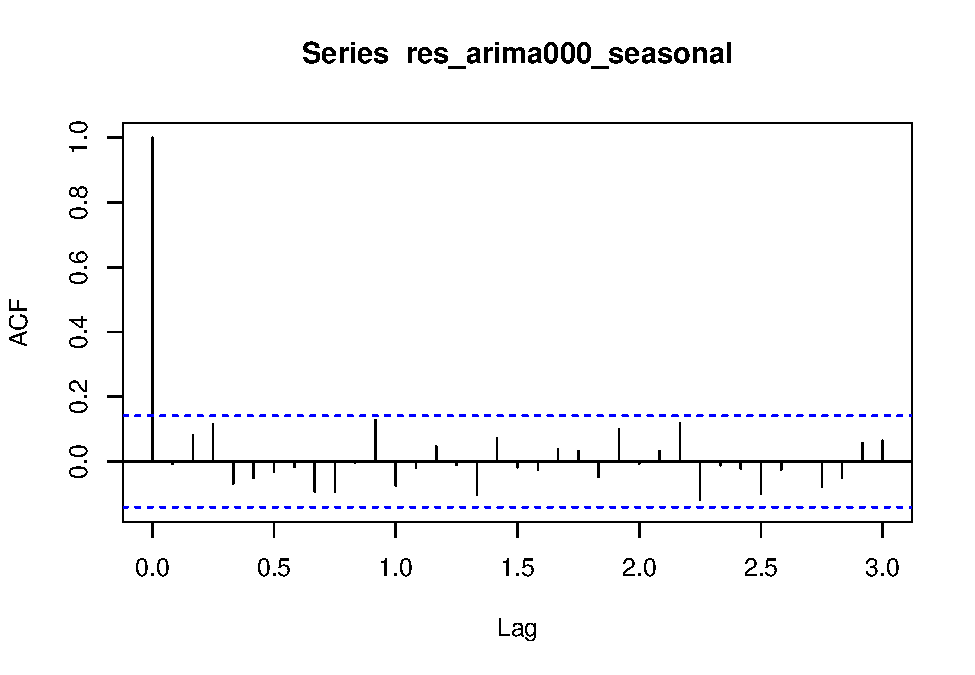
\includegraphics{final_sixth_meetings_notes_files/figure-latex/unnamed-chunk-3-1.pdf}

As it turns out, the ARIMA(1,0,0) and ARIMA(0,1,0) do not return the
same ACF plots. The ACF at lag 1 of the ARIMA(0,1,0) is negative.

\hypertarget{arima010-with-constant}{%
\subsection{ARIMA(0,1,0) with constant}\label{arima010-with-constant}}

\begin{Shaded}
\begin{Highlighting}[]
\NormalTok{bx\_arima010\_fit }\OtherTok{\textless{}{-}}\NormalTok{ bx\_ts }\SpecialCharTok{\%\textgreater{}\%} \FunctionTok{model}\NormalTok{(}\AttributeTok{arima010\_constant =} \FunctionTok{ARIMA}\NormalTok{(total\_waste }\SpecialCharTok{\textasciitilde{}} \DecValTok{1} \SpecialCharTok{+} \FunctionTok{pdq}\NormalTok{(}\DecValTok{0}\NormalTok{,}\DecValTok{1}\NormalTok{,}\DecValTok{0}\NormalTok{)))}
\end{Highlighting}
\end{Shaded}

\begin{Shaded}
\begin{Highlighting}[]
\NormalTok{bx\_arima010\_fit}\SpecialCharTok{\%\textgreater{}\%} \FunctionTok{gg\_tsresiduals}\NormalTok{(}\AttributeTok{lag =} \DecValTok{24}\NormalTok{)}
\end{Highlighting}
\end{Shaded}

\includegraphics{final_sixth_meetings_notes_files/figure-latex/ACF plot-1.pdf}

From the ACF, we see significant values at lag (1, 13), and positive
significant values at lag (12). A ``sharp cutoff'' is subjective here.
Lags 2 and 3 are small, but then the ACF values picks up again on lag 4.

\begin{Shaded}
\begin{Highlighting}[]
\NormalTok{bx\_ts }\SpecialCharTok{\%\textgreater{}\%} \FunctionTok{gg\_tsdisplay}\NormalTok{(diff1, }\AttributeTok{plot\_type =} \StringTok{"partial"}\NormalTok{)}
\end{Highlighting}
\end{Shaded}

\begin{verbatim}
## Warning: Removed 1 row(s) containing missing values (geom_path).
\end{verbatim}

\begin{verbatim}
## Warning: Removed 1 rows containing missing values (geom_point).
\end{verbatim}

\includegraphics{final_sixth_meetings_notes_files/figure-latex/PACF Plot-1.pdf}

The PACF displays significant lag values at lags (1, 2,4, 10, 11).

From the DUKE Arima study
\href{https://people.duke.edu/~rnau/411arim3.htm}{guide}, ``An MA
signature is commonly associated with negative autocorrelation at lag
1--i.e., it tends to arise in series which are slightly overdifferenced.
The reason for this is that an MA term can''partially cancel'' an order
of differencing in the forecasting equation.''

\hypertarget{for-now-i-will-skip-the-attemps-at-adding-ar-parameters-as-i-will-focus-on-getting-the-acf-values-close-to-zero-with-ma-parameters}{%
\paragraph{For now, I will skip the attemps at adding AR() parameters,
as I will focus on getting the ACF values close to zero with MA()
parameters}\label{for-now-i-will-skip-the-attemps-at-adding-ar-parameters-as-i-will-focus-on-getting-the-acf-values-close-to-zero-with-ma-parameters}}

\hypertarget{arima001-with-out-a-constant}{%
\subsection{ARIMA(0,0,1) with out a
constant}\label{arima001-with-out-a-constant}}

\includegraphics{final_sixth_meetings_notes_files/figure-latex/ARIMA(001) no constant-1.pdf}

We see that the first ACF value is not significant and is positive.
Lags(2, 12, 24) are significant. There appears to be a seasonal
component, as evident from lags 12 and 24.

\begin{Shaded}
\begin{Highlighting}[]
\NormalTok{bx\_arima001\_fit }\SpecialCharTok{\%\textgreater{}\%} \FunctionTok{forecast}\NormalTok{(}\AttributeTok{h =} \DecValTok{8}\NormalTok{) }\CommentTok{\#the estimates immediately stabilizes}
\end{Highlighting}
\end{Shaded}

\begin{verbatim}
## # A fable: 8 x 4 [1]
## # Key:     .model [1]
##   .model   month_num       total_waste  .mean
##   <chr>        <dbl>            <dist>  <dbl>
## 1 arima001       193 N(42460, 8142967) 42460.
## 2 arima001       194 N(41208, 8796266) 41208.
## 3 arima001       195 N(41208, 8796266) 41208.
## 4 arima001       196 N(41208, 8796266) 41208.
## 5 arima001       197 N(41208, 8796266) 41208.
## 6 arima001       198 N(41208, 8796266) 41208.
## 7 arima001       199 N(41208, 8796266) 41208.
## 8 arima001       200 N(41208, 8796266) 41208.
\end{verbatim}

\begin{Shaded}
\begin{Highlighting}[]
\NormalTok{bx\_arima001\_fit }\SpecialCharTok{\%\textgreater{}\%} \FunctionTok{forecast}\NormalTok{(}\AttributeTok{h =} \DecValTok{8}\NormalTok{) }\SpecialCharTok{\%\textgreater{}\%} \FunctionTok{autoplot}\NormalTok{(bx\_ts)}
\end{Highlighting}
\end{Shaded}

\includegraphics{final_sixth_meetings_notes_files/figure-latex/forecast-1.pdf}

\hypertarget{arima012-with-out-a-constant}{%
\subsection{ARIMA(0,1,2) with out a
constant}\label{arima012-with-out-a-constant}}

\begin{Shaded}
\begin{Highlighting}[]
\NormalTok{bx\_arima012\_fit }\OtherTok{\textless{}{-}}\NormalTok{ bx\_ts }\SpecialCharTok{\%\textgreater{}\%} \FunctionTok{model}\NormalTok{(}\AttributeTok{arima012 =} \FunctionTok{ARIMA}\NormalTok{(total\_waste }\SpecialCharTok{\textasciitilde{}} \FunctionTok{pdq}\NormalTok{(}\DecValTok{0}\NormalTok{,}\DecValTok{1}\NormalTok{,}\DecValTok{2}\NormalTok{)))}
\NormalTok{bx\_arima012\_fit }\SpecialCharTok{\%\textgreater{}\%} \FunctionTok{gg\_tsresiduals}\NormalTok{(}\AttributeTok{lag =} \DecValTok{24}\NormalTok{)}
\end{Highlighting}
\end{Shaded}

\includegraphics{final_sixth_meetings_notes_files/figure-latex/ARIMA(0,1,2) no constant \& residuals plot-1.pdf}

From the ACF plot, we can see that the first significant lag begins at
lag 12. The lags (2, 4, 8) barely pass the significance threshold.

\begin{Shaded}
\begin{Highlighting}[]
\NormalTok{bx\_arima012\_fit }\SpecialCharTok{\%\textgreater{}\%} \FunctionTok{forecast}\NormalTok{(}\AttributeTok{h =} \DecValTok{8}\NormalTok{) }\SpecialCharTok{\%\textgreater{}\%} \FunctionTok{autoplot}\NormalTok{(bx\_ts)}
\end{Highlighting}
\end{Shaded}

\includegraphics{final_sixth_meetings_notes_files/figure-latex/forecast plot2-1.pdf}

\hypertarget{arima012-with-a-seasonal-parameter-and-period-12}{%
\subsection{ARIMA(0,1,2) with a seasonal parameter and period =
12}\label{arima012-with-a-seasonal-parameter-and-period-12}}

More
\href{https://fable.tidyverts.org/reference/ARIMA.html}{information} on
the parameter selection.

\hypertarget{this-is-the-one-i-like-the-most}{%
\subsubsection{This is the one I like the
most}\label{this-is-the-one-i-like-the-most}}

\begin{Shaded}
\begin{Highlighting}[]
\NormalTok{bx\_arima012\_001\_12 }\OtherTok{\textless{}{-}}\NormalTok{ bx\_ts }\SpecialCharTok{\%\textgreater{}\%} \FunctionTok{model}\NormalTok{(}\AttributeTok{bx\_arima012\_001\_12 =} \FunctionTok{ARIMA}\NormalTok{(total\_waste }\SpecialCharTok{\textasciitilde{}} \FunctionTok{pdq}\NormalTok{(}\DecValTok{0}\NormalTok{,}\DecValTok{1}\NormalTok{,}\DecValTok{2}\NormalTok{) }\SpecialCharTok{+} \FunctionTok{PDQ}\NormalTok{(}\DecValTok{0}\NormalTok{,}\DecValTok{0}\NormalTok{,}\DecValTok{1}\NormalTok{, }\AttributeTok{period =} \DecValTok{12}\NormalTok{)))}
\NormalTok{bx\_arima012\_001\_12 }\SpecialCharTok{\%\textgreater{}\%} \FunctionTok{gg\_tsresiduals}\NormalTok{(}\AttributeTok{lag =} \DecValTok{36}\NormalTok{)}
\end{Highlighting}
\end{Shaded}

\includegraphics{final_sixth_meetings_notes_files/figure-latex/ARIMA fit-1.pdf}

\begin{Shaded}
\begin{Highlighting}[]
\NormalTok{bx\_arima012\_001\_12 }\SpecialCharTok{\%\textgreater{}\%} \FunctionTok{report}\NormalTok{()}
\end{Highlighting}
\end{Shaded}

\begin{verbatim}
## Series: total_waste 
## Model: ARIMA(0,1,2)(0,0,1)[12] 
## 
## Coefficients:
##           ma1      ma2    sma1
##       -0.7227  -0.1173  0.4361
## s.e.   0.0683   0.0738  0.0621
## 
## sigma^2 estimated as 6251155:  log likelihood=-1765.68
## AIC=3539.36   AICc=3539.58   BIC=3552.37
\end{verbatim}

With a ``1'', order of the seasonal moving average (SMA) terms and a
period of 12, we get all ACF values except for 24 to within the 95\%
intervals.

\hypertarget{arima012-with-no-seasonal-parameter-and-period-12}{%
\subsection{ARIMA(0,1,2) with no seasonal parameter and period =
12}\label{arima012-with-no-seasonal-parameter-and-period-12}}

\begin{Shaded}
\begin{Highlighting}[]
\NormalTok{bx\_arima012\_000\_12 }\OtherTok{\textless{}{-}}\NormalTok{ bx\_ts }\SpecialCharTok{\%\textgreater{}\%} \FunctionTok{model}\NormalTok{(}\AttributeTok{bx\_arima012\_000\_12 =} \FunctionTok{ARIMA}\NormalTok{(total\_waste }\SpecialCharTok{\textasciitilde{}} \FunctionTok{pdq}\NormalTok{(}\DecValTok{0}\NormalTok{,}\DecValTok{1}\NormalTok{,}\DecValTok{2}\NormalTok{) }\SpecialCharTok{+} \FunctionTok{PDQ}\NormalTok{(}\DecValTok{0}\NormalTok{,}\DecValTok{0}\NormalTok{,}\DecValTok{0}\NormalTok{, }\AttributeTok{period =} \DecValTok{12}\NormalTok{)))}
\NormalTok{bx\_arima012\_000\_12 }\SpecialCharTok{\%\textgreater{}\%} \FunctionTok{gg\_tsresiduals}\NormalTok{(}\AttributeTok{lag =} \DecValTok{36}\NormalTok{)}
\end{Highlighting}
\end{Shaded}

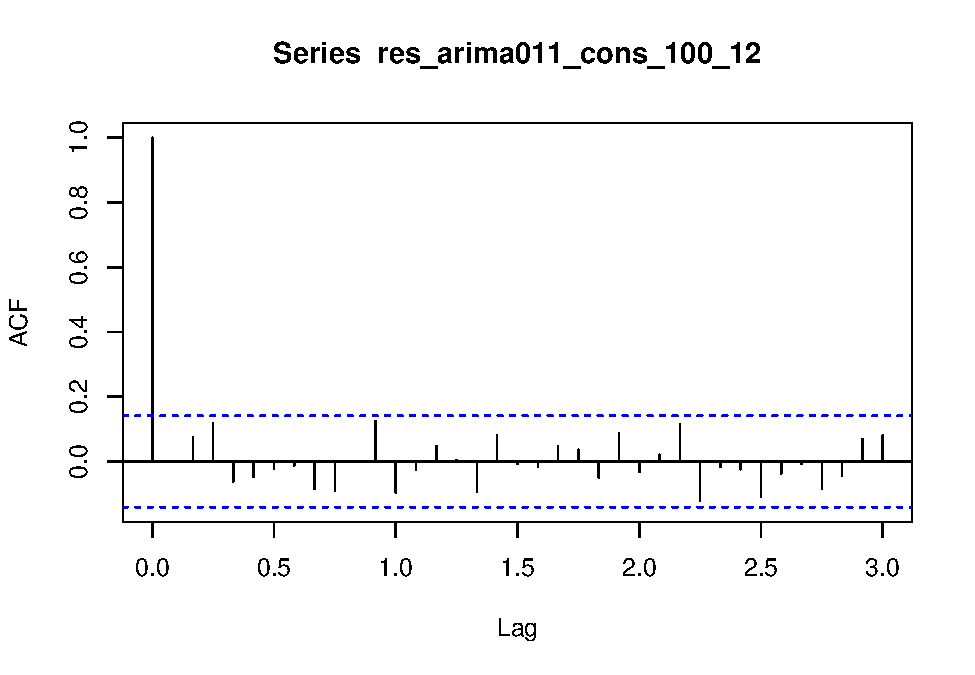
\includegraphics{final_sixth_meetings_notes_files/figure-latex/unnamed-chunk-4-1.pdf}

\begin{Shaded}
\begin{Highlighting}[]
\NormalTok{bx\_arima012\_000\_12 }\SpecialCharTok{\%\textgreater{}\%} \FunctionTok{report}\NormalTok{()}
\end{Highlighting}
\end{Shaded}

\begin{verbatim}
## Series: total_waste 
## Model: ARIMA(0,1,2) 
## 
## Coefficients:
##          ma1      ma2
##       -0.699  -0.1745
## s.e.   0.066   0.0655
## 
## sigma^2 estimated as 7778282:  log likelihood=-1785.96
## AIC=3577.92   AICc=3578.04   BIC=3587.67
\end{verbatim}

The ACF values at lag 12 is significant. And the MA() arguments add up
to equal to 0.86.

Section \href{https://otexts.com/fpp3/seasonal-arima.html}{9.9} of the
fpp3 textbook makes a claim that ``an
\(\text{ARIMA(0,0,0)(0,0,1)}_{12}\) model will show:

\begin{itemize}
\tightlist
\item
  a spike at lag 12 in the ACF but no other significant spikes;
\item
  exponential decay in the seasonal lags of the PACF (i.e., at lags 12,
  24, 36, \ldots).''
\end{itemize}

\begin{Shaded}
\begin{Highlighting}[]
\NormalTok{bx\_arima000\_001\_12 }\OtherTok{\textless{}{-}}\NormalTok{ bx\_ts }\SpecialCharTok{\%\textgreater{}\%} \FunctionTok{model}\NormalTok{(}\AttributeTok{arima012\_no\_ma\_seasonal =} \FunctionTok{ARIMA}\NormalTok{(total\_waste }\SpecialCharTok{\textasciitilde{}} \FunctionTok{pdq}\NormalTok{(}\DecValTok{0}\NormalTok{,}\DecValTok{0}\NormalTok{,}\DecValTok{0}\NormalTok{) }\SpecialCharTok{+} \FunctionTok{PDQ}\NormalTok{(}\DecValTok{0}\NormalTok{,}\DecValTok{0}\NormalTok{,}\DecValTok{1}\NormalTok{, }\AttributeTok{period =} \DecValTok{12}\NormalTok{))) }
\NormalTok{bx\_arima000\_001\_12 }\SpecialCharTok{\%\textgreater{}\%} \FunctionTok{gg\_tsresiduals}\NormalTok{(}\AttributeTok{lag =} \DecValTok{36}\NormalTok{)}
\end{Highlighting}
\end{Shaded}

\includegraphics{final_sixth_meetings_notes_files/figure-latex/unnamed-chunk-5-1.pdf}

\begin{Shaded}
\begin{Highlighting}[]
\NormalTok{bx\_arima000\_001\_12 }\SpecialCharTok{\%\textgreater{}\%} \FunctionTok{report}\NormalTok{()}
\end{Highlighting}
\end{Shaded}

\begin{verbatim}
## Series: total_waste 
## Model: ARIMA(0,0,0)(0,0,1)[12] w/ mean 
## 
## Coefficients:
##         sma1    constant
##       0.4746  41335.3762
## s.e.  0.0637    276.5976
## 
## sigma^2 estimated as 7073688:  log likelihood=-1787.06
## AIC=3580.13   AICc=3580.26   BIC=3589.9
\end{verbatim}

In our data, we do not see this as the the first three lags return
significant ACF values. Then again at lag 24. The SMA() parameter is
approximately 0.47, with the constant approximating 41,335.

The authors make a similar claim with ``an
\(\text{ARIMA(0,0,0)(1,0,0)}_{12}\) model will show:

\begin{itemize}
\tightlist
\item
  exponential decay in the seasonal lags of the ACF;
\item
  a single significant spike at lag 12 in the PACF.''
\end{itemize}

\begin{Shaded}
\begin{Highlighting}[]
\NormalTok{bx\_arima000\_100\_12 }\OtherTok{\textless{}{-}}\NormalTok{ bx\_ts }\SpecialCharTok{\%\textgreater{}\%} \FunctionTok{model}\NormalTok{(}\AttributeTok{arima012\_no\_ma\_seasonal =} \FunctionTok{ARIMA}\NormalTok{(total\_waste }\SpecialCharTok{\textasciitilde{}} \FunctionTok{pdq}\NormalTok{(}\DecValTok{0}\NormalTok{,}\DecValTok{0}\NormalTok{,}\DecValTok{0}\NormalTok{) }\SpecialCharTok{+} \FunctionTok{PDQ}\NormalTok{(}\DecValTok{1}\NormalTok{,}\DecValTok{0}\NormalTok{,}\DecValTok{0}\NormalTok{, }\AttributeTok{period =} \DecValTok{12}\NormalTok{))) }
\NormalTok{bx\_arima000\_100\_12 }\SpecialCharTok{\%\textgreater{}\%} \FunctionTok{gg\_tsresiduals}\NormalTok{(}\AttributeTok{lag =} \DecValTok{36}\NormalTok{)}
\end{Highlighting}
\end{Shaded}

\includegraphics{final_sixth_meetings_notes_files/figure-latex/unnamed-chunk-6-1.pdf}

\begin{Shaded}
\begin{Highlighting}[]
\NormalTok{bx\_arima000\_100\_12 }\SpecialCharTok{\%\textgreater{}\%} \FunctionTok{report}\NormalTok{()}
\end{Highlighting}
\end{Shaded}

\begin{verbatim}
## Series: total_waste 
## Model: ARIMA(0,0,0)(1,0,0)[12] w/ mean 
## 
## Coefficients:
##         sar1    constant
##       0.6108  16188.9677
## s.e.  0.0644    167.3437
## 
## sigma^2 estimated as 6223989:  log likelihood=-1776.05
## AIC=3558.1   AICc=3558.23   BIC=3567.87
\end{verbatim}

Again, the first three lags return significant ACF values, but there is
exponential decay in the seasonal lags of the ACF. The SAR() parameter
approximates 0.61, with the constant approximating 16188.

\begin{Shaded}
\begin{Highlighting}[]
\NormalTok{bx\_ts }\SpecialCharTok{\%\textgreater{}\%} 
  \FunctionTok{gg\_tsdisplay}\NormalTok{(}\FunctionTok{difference}\NormalTok{(total\_waste, }\DecValTok{12}\NormalTok{),}
               \AttributeTok{plot\_type =} \StringTok{"partial"}\NormalTok{, }\AttributeTok{lag =} \DecValTok{36}\NormalTok{) }\SpecialCharTok{+}
  \FunctionTok{labs}\NormalTok{(}\AttributeTok{title =} \StringTok{"Seasonally Differenced"}\NormalTok{, }\AttributeTok{y =} \StringTok{""}\NormalTok{)}
\end{Highlighting}
\end{Shaded}

\begin{verbatim}
## Warning: Removed 12 row(s) containing missing values (geom_path).
\end{verbatim}

\begin{verbatim}
## Warning: Removed 12 rows containing missing values (geom_point).
\end{verbatim}

\includegraphics{final_sixth_meetings_notes_files/figure-latex/unnamed-chunk-7-1.pdf}

\begin{Shaded}
\begin{Highlighting}[]
\NormalTok{bx\_ts }\SpecialCharTok{\%\textgreater{}\%} 
  \FunctionTok{gg\_tsdisplay}\NormalTok{(}\FunctionTok{difference}\NormalTok{(total\_waste, }\DecValTok{12}\NormalTok{) }\SpecialCharTok{\%\textgreater{}\%} \FunctionTok{difference}\NormalTok{(),}
               \AttributeTok{plot\_type =} \StringTok{"partial"}\NormalTok{, }\AttributeTok{lag =} \DecValTok{36}\NormalTok{) }\SpecialCharTok{+}
  \FunctionTok{labs}\NormalTok{(}\AttributeTok{title =} \StringTok{"Double Differenced"}\NormalTok{, }\AttributeTok{y =} \StringTok{""}\NormalTok{)}
\end{Highlighting}
\end{Shaded}

\begin{verbatim}
## Warning: Removed 13 row(s) containing missing values (geom_path).
\end{verbatim}

\begin{verbatim}
## Warning: Removed 13 rows containing missing values (geom_point).
\end{verbatim}

\includegraphics{final_sixth_meetings_notes_files/figure-latex/unnamed-chunk-8-1.pdf}

\hypertarget{this-is-my-second-favorite-model-with-no-seasonal-difference-needed-and-most-of-the-acf-values-are-not-significant.}{%
\subsubsection{This is my second favorite model, with no seasonal
difference needed and most of the ACF values are not
significant.}\label{this-is-my-second-favorite-model-with-no-seasonal-difference-needed-and-most-of-the-acf-values-are-not-significant.}}

The significant spike at lag 1 in the ACF suggests a non-seasonal MA(1)
component. The significant spike at lag 12 in the ACF suggests a
seasonal MA(1) component.

\begin{Shaded}
\begin{Highlighting}[]
\NormalTok{bx\_arima011\_001\_12 }\OtherTok{\textless{}{-}}\NormalTok{ bx\_ts }\SpecialCharTok{\%\textgreater{}\%} \FunctionTok{model}\NormalTok{(}\AttributeTok{bx\_arima011\_001\_12 =} \FunctionTok{ARIMA}\NormalTok{(total\_waste }\SpecialCharTok{\textasciitilde{}} \FunctionTok{pdq}\NormalTok{(}\DecValTok{0}\NormalTok{,}\DecValTok{1}\NormalTok{,}\DecValTok{1}\NormalTok{) }\SpecialCharTok{+} \FunctionTok{PDQ}\NormalTok{(}\DecValTok{0}\NormalTok{,}\DecValTok{0}\NormalTok{,}\DecValTok{1}\NormalTok{, }\AttributeTok{period =} \DecValTok{12}\NormalTok{))) }
\NormalTok{bx\_arima011\_001\_12 }\SpecialCharTok{\%\textgreater{}\%} \FunctionTok{gg\_tsresiduals}\NormalTok{()}
\end{Highlighting}
\end{Shaded}

\includegraphics{final_sixth_meetings_notes_files/figure-latex/unnamed-chunk-9-1.pdf}

\begin{Shaded}
\begin{Highlighting}[]
\NormalTok{bx\_arima011\_001\_12 }\SpecialCharTok{\%\textgreater{}\%}\NormalTok{ report}
\end{Highlighting}
\end{Shaded}

\begin{verbatim}
## Series: total_waste 
## Model: ARIMA(0,1,1)(0,0,1)[12] 
## 
## Coefficients:
##           ma1    sma1
##       -0.7728  0.4563
## s.e.   0.0733  0.0607
## 
## sigma^2 estimated as 6293078:  log likelihood=-1766.9
## AIC=3539.79   AICc=3539.92   BIC=3549.55
\end{verbatim}

\hypertarget{creating-the-final-fitted-model-with-5-arima-models}{%
\subsection{Creating the final fitted model with 5 ARIMA
models}\label{creating-the-final-fitted-model-with-5-arima-models}}

\begin{Shaded}
\begin{Highlighting}[]
\NormalTok{bx\_arima\_fit }\OtherTok{\textless{}{-}}\NormalTok{ bx\_ts }\SpecialCharTok{\%\textgreater{}\%} \FunctionTok{model}\NormalTok{(}\AttributeTok{arma100 =} \FunctionTok{ARIMA}\NormalTok{(total\_waste }\SpecialCharTok{\textasciitilde{}} \FunctionTok{pdq}\NormalTok{(}\DecValTok{1}\NormalTok{,}\DecValTok{0}\NormalTok{,}\DecValTok{0}\NormalTok{)),}
                \AttributeTok{arima010 =} \FunctionTok{ARIMA}\NormalTok{(total\_waste }\SpecialCharTok{\textasciitilde{}} \FunctionTok{pdq}\NormalTok{(}\DecValTok{0}\NormalTok{,}\DecValTok{1}\NormalTok{,}\DecValTok{0}\NormalTok{)),}
                \AttributeTok{arima001 =} \FunctionTok{ARIMA}\NormalTok{(total\_waste }\SpecialCharTok{\textasciitilde{}} \FunctionTok{pdq}\NormalTok{(}\DecValTok{0}\NormalTok{,}\DecValTok{0}\NormalTok{,}\DecValTok{1}\NormalTok{)),}
                \AttributeTok{arima012\_001\_12 =} \FunctionTok{ARIMA}\NormalTok{(total\_waste }\SpecialCharTok{\textasciitilde{}} \FunctionTok{pdq}\NormalTok{(}\DecValTok{0}\NormalTok{,}\DecValTok{1}\NormalTok{,}\DecValTok{2}\NormalTok{) }\SpecialCharTok{+} \FunctionTok{PDQ}\NormalTok{(}\DecValTok{0}\NormalTok{,}\DecValTok{0}\NormalTok{,}\DecValTok{1}\NormalTok{, }\AttributeTok{period =} \DecValTok{12}\NormalTok{)),}
                \AttributeTok{arima011\_001\_12 =} \FunctionTok{ARIMA}\NormalTok{(total\_waste }\SpecialCharTok{\textasciitilde{}} \FunctionTok{pdq}\NormalTok{(}\DecValTok{0}\NormalTok{,}\DecValTok{1}\NormalTok{,}\DecValTok{1}\NormalTok{) }\SpecialCharTok{+} \FunctionTok{PDQ}\NormalTok{(}\DecValTok{0}\NormalTok{,}\DecValTok{0}\NormalTok{,}\DecValTok{1}\NormalTok{, }\AttributeTok{period =} \DecValTok{12}\NormalTok{)))}
\end{Highlighting}
\end{Shaded}

\hypertarget{forecast-plot-along-with-accuracy-metrics-and-model}{%
\subsubsection{Forecast plot, along with accuracy metrics and
model}\label{forecast-plot-along-with-accuracy-metrics-and-model}}

\begin{Shaded}
\begin{Highlighting}[]
\NormalTok{bx\_arima\_fit }\SpecialCharTok{\%\textgreater{}\%} \FunctionTok{forecast}\NormalTok{(}\AttributeTok{h =} \DecValTok{8}\NormalTok{) }\SpecialCharTok{\%\textgreater{}\%} \FunctionTok{autoplot}\NormalTok{(bx\_ts) }\SpecialCharTok{+} \FunctionTok{labs}\NormalTok{(}\AttributeTok{x =} \StringTok{"Month Number"}\NormalTok{, }
                                                            \AttributeTok{y =} \StringTok{"Total Waste Tonnage"}\NormalTok{)}
\end{Highlighting}
\end{Shaded}

\includegraphics{final_sixth_meetings_notes_files/figure-latex/unnamed-chunk-11-1.pdf}

\begin{Shaded}
\begin{Highlighting}[]
\FunctionTok{accuracy}\NormalTok{(bx\_arima\_fit) }\SpecialCharTok{|}\ErrorTok{\textgreater{}} \FunctionTok{arrange}\NormalTok{(}\StringTok{"RMSE"}\NormalTok{)}
\end{Highlighting}
\end{Shaded}

\begin{verbatim}
## # A tibble: 5 x 10
##   .model          .type        ME  RMSE   MAE      MPE  MAPE  MASE RMSSE    ACF1
##   <chr>           <chr>     <dbl> <dbl> <dbl>    <dbl> <dbl> <dbl> <dbl>   <dbl>
## 1 arma100         Traini~   4.48  2770. 2038. -4.63e-1  5.06 0.804 0.833 -0.0713
## 2 arima010        Traini~  36.1   3317. 2522. -2.63e-1  6.25 0.995 0.997 -0.443 
## 3 arima001        Traini~   0.618 2839. 2108. -5.02e-1  5.22 0.832 0.854  0.0642
## 4 arima012_001_12 Traini~ 164.    2474. 1755.  2.53e-2  4.31 0.692 0.744  0.0110
## 5 arima011_001_12 Traini~ 151.    2489. 1771. -8.79e-4  4.36 0.699 0.748  0.0792
\end{verbatim}

\begin{Shaded}
\begin{Highlighting}[]
\FunctionTok{glance}\NormalTok{(bx\_arima\_fit) }\SpecialCharTok{\%\textgreater{}\%} 
  \FunctionTok{arrange}\NormalTok{(AICc) }\SpecialCharTok{\%\textgreater{}\%} 
  \FunctionTok{select}\NormalTok{(.model}\SpecialCharTok{:}\NormalTok{BIC)}
\end{Highlighting}
\end{Shaded}

\begin{verbatim}
## # A tibble: 5 x 6
##   .model             sigma2 log_lik   AIC  AICc   BIC
##   <chr>               <dbl>   <dbl> <dbl> <dbl> <dbl>
## 1 arima012_001_12  6251155.  -1766. 3539. 3540. 3552.
## 2 arima011_001_12  6293078.  -1767. 3540. 3540. 3550.
## 3 arma100          7752732.  -1794. 3595. 3595. 3605.
## 4 arima001         8142967.  -1799. 3604. 3604. 3614.
## 5 arima010        11059715.  -1820. 3642. 3642. 3645.
\end{verbatim}

The model with the lowest RMSE is the
\(\text{ARIMA(0,1,2)(0,0,1)}_{12}\) and
\(\text{ARIMA(0,1,1)(0,0,1)}_{12}\) .

\hypertarget{individual-forecast-plot-of-the-best-performing-models}{%
\subsubsection{Individual forecast plot of the best performing
models}\label{individual-forecast-plot-of-the-best-performing-models}}

\begin{Shaded}
\begin{Highlighting}[]
\NormalTok{bx\_arima\_fit }\SpecialCharTok{\%\textgreater{}\%} \FunctionTok{select}\NormalTok{(}\AttributeTok{.model =} \FunctionTok{c}\NormalTok{(arima011\_001\_12, arima012\_001\_12)) }\SpecialCharTok{\%\textgreater{}\%} \FunctionTok{forecast}\NormalTok{(}\AttributeTok{h =} \DecValTok{8}\NormalTok{) }\SpecialCharTok{\%\textgreater{}\%} \FunctionTok{autoplot}\NormalTok{(bx\_ts)}
\end{Highlighting}
\end{Shaded}

\includegraphics{final_sixth_meetings_notes_files/figure-latex/unnamed-chunk-12-1.pdf}

\begin{Shaded}
\begin{Highlighting}[]
\CommentTok{\# bx\_arima\_fit \%\textgreater{}\% filter(.model == arima011\_001\_12) \%\textgreater{}\% forecast(h = 8) \%\textgreater{}\% autoplot(bx\_ts) + labs(x = "Month Number", y = "Total Waste Tonnage")}
\end{Highlighting}
\end{Shaded}


\end{document}
